%\documentclass{report}\begin{document}
\chapter{Group Theory (\textit{Not done})}

\myTop{In this chapter we will explain group theory and how it can be used to solve the \rubik{}. When we have a good understanding of the group theory we will be able to use it later for our own program.
}

\section{Permutations}
In this section we will use the same move notations as in \ref{sec:moveNotation}.
To calculate how many positions the cube can be placed in, we have to look at the general cube terminology \ref{sec:generalNotation}.
As stated in general cube terminology there is 8 corners \cpiece{} and the first corner you place can be placed in 8 positions, and after that is placed the next corner \cpiece{} can be placed in one of the 7 positions left, since we already use 1, and so on. So that means that the corner pieces can be placed in $8\cdot7\cdot6\cdot5\cdot4\cdot3\cdot2\cdot1=8!$ positions. Now the 8 corner \cpiece{} is placed at the right position they might not have the right orientation since a corner \cpiece{} has three different colors and therefor 3 different orientations, so there are $3^8$ orientations of the 8 corner \cpiece{}. That means there is $8!\cdot3^8$ ways the corner \cpiece{} can be placed. As stated in the terminology there are 12 edge \cpiece{}s. These edge \cpiece{}s can be positioned in 12 different positions and every edge \cpiece{} can be oriented in two different ways. So there is $2^12$ different orientations and $12!$ different positions of the edge \cpiece{}. This gives us $2^{12}\cdot12!$ different edge permutations and a total of $3^8\cdot2^{12}\cdot12!\cdot8!=519,024,039,293,878,272,000$

\section{Definition of the Rubik's Cube group}
To fully understand if the \rubik{} can be described as group theory, it will be needed to understand what a group is.
To describe a group in group theory the group is written $(Element, Operator)$ where the element is the sets the group consist of and the operator is the operation that is made between the sets. When the \rubik{} is made into a group the set will be a move or a set of moves that are applied to the \rubik{}. The operator in the \rubik{} group will be astrix (*) because the \rubik{}s movements are not commutative. They are not commutative because it does not matter in which order the moves is applied to the \rubik{}\cite[p. 157]{Rubik87} .

To prove that the \rubik{} is a group there is four points it must fullfill:

\begin {itemize}
\item When two elements is combined with an operation then the new element these creates must also be a part of the group. For instance a move $M_1$ and a move $M_2$ then $M_1 * M_2$ will form a new move or move sequence which also is a part of the group.

\item $e$ is an empty move (which does not change the configuration of the \rubik{}), So if you have to do the move $M * e$ that basicly means that you have the move $M$ and then do nothing (this could be a $360^o$ twist of a face), so that means that $M*e=M$

\item If $M$ is a move then it is possible to reverse this move, this moved is called $M'$. Therefore $M*M' = e$, so every elements in the group has a reverse move.

%Følgende punkt skal lige laves noget smart ved.
\item To prove $*$ is associative it is important to remember that the moves made on the \rubik{} can be defined on the changes it makes to the configuration of the \rubik{}. 
If $c$ is an oriented rubik's cubie, $M(c)$ will be the orientation $c$ for the oriented cubicle $c$ ends in after the move is applied.
Example the move $R$ wll move the $ur$ cubie to the $br$ cubicle, so therefore $R(ur)=br$. If there is more than one move sequence then the operation will look like this $B'(R(ur))=db$. If there is another move the cubie will be oriented in the $M_2 (M_1 (c))$, therefore $(M_1 *M_2 )(c)=M_2 (M_1 (c))$. 

\end {itemize}

$*$ is associative (samme som not commutative?) because $(M_1 *M_2 )*M_3 = M_1 *(M_2 *M_3 )$ for any moves $M_1$, $M_2$ and $M_3$. $(M_1 *M_2 )*M_3$ and $M_1 *(M_2 *M_3 )$ does the same operation to every cubie. This is the same as saying $[(M_1 *M_2 )*M_3 ](C)=[M_1 *(M_2 *M_3 )](C)=M_3 (M_2 (M_1 (C)))$ for any cubie $C$. Therefore $*$ is associative.


\section{Subgroup}
As said in the Permutation section, there is $3^8*2^{12}*12!*8!$ possible configurations, but it is not all of these configurations that are possible to do.  To make it more easy there will only be looked at some moves of the \rubik{} but only the moves of the down and right faces. To better understand G, it can be split up in small pieces.
A nonempty subset H of the group (G,*) is called a subgroup of G if (H,*) is a group
To check if a subset actually is a subgroup the following can be used.


Let $(G,*)$ be a group. A nonempty subset $H$ of $G$ is a subgroup of $(G,*)$ iff, for every $a, b \in H$, $a * b^(-1) \in H$.

Proof. First, suppose $H$ is a subgroup. If $b \in H$, then $b^(-1) \in H since (H,*)$ is a group. So, if $a \in H$ as well, then $a * b^(-1) \in H$.

Conversely, suppose that, for every $a, b \in H$, $a * b^(-1) \in H$.

\begin {itemize}
\item First, notice that $*$ is associative since $(G,*)$ is a group.
\item Let $a \in H$. Then, $e = a * a^(-1)$, so $e \in H$.
\item Let $b \in H$. Then $b^(-1) = e * b^(-1) \in H$, so inverse exist in $H$.
\item Let $a, b \in H$. By the previous step, $b^(-1) \in H$, so $a* (b^(-1))^(-1) = a* b \in H$. Thus, $H$ is closed under $*$.
\end {itemize}

Therefore, $(H,*)$ is a group, which means that $H$ is a subgroup of $G$.

\section{The Symmetric Group}

Instead of just looking at configurations of 8 cubies, the configurations of the cube can be seen as $n$ objects. 
These objects be named $1, 2, . . . , n,$ these names are arbitrary. the arranging of these objects can be seen as
putting them into $n$ slots. If the slots is numberet $1, 2, . . . , n,$ can it be define as a function $\sigma : {1, 2, . . . , n} \rightarrow
{1, 2, . . . , n}$ by letting $\sigma(i)$ be the number put into slot $i$.

\subsection{Example} 
Tag the objects $1, 2, 3$ in the order $3 1 2$. So, it corresponds to the function $\sigma: {1, 2, 3} \rightarrow {1, 2, 3}$
defined by $\sigma(1) = 3$,$\sigma(2) = 1$, and $\sigma(3) = 2$.

\subsection{Lemma}

Imagine that $x\neq y$. Since a number cannot be in more than one slot, if $x \neq y$, slots x and y must contain

different numbers. That is, $\sigma(x) \neq \sigma(y)$. Therefore, $\sigma$ is one-to-one.

Any number $y \in {1, 2, . . . , n}$ must lie in some slot, say slot x. Then, $\sigma(x) = y$.

But if $\sigma: {1, . . . , n} \rightarrow {1, . . . , n}$ is a bijection, So $\sigma$ can be used to defines the arrangement of the n
objects: just put object $\sigma(i)$ in slot i. So, the arrangements is the same as the set of
bijections ${1, . . . , n} \rightarrow {1, . . . , n}$. Therefore, instead of studying possible arrangements, the bijections can be studied instead.

\subsection{Definition}

The Symmetric Group of $n$ letters are the set of bijection from ${1,2,......n}$ to ${1,2,......n}$ with the operation of composition. This group will be called $S_n$

\subsection{Exemple}

Let $\sigma,\tau \neq S_3$ be defined as $\sigma(1)=3, \sigma(2)=1, \sigma(3)=2, \tau(1)=1,\tau(2)=3,\tau(3)=2$ so $(\sigma\tau)(1)=\tau(3)=2,(\sigma\tau)(2)=\tau(1)=1, (\sigma\tau)(3)=\tau(2)=3.$

\section{Disjoint Cycle Decomposition}

There is a more compact way of writing elements of the symmetric group; this can best be explained by an
example.

\subsection{Example} Consider $\sigma \in S_(12)$ defined by

	$\sigma(1) = 12 \sigma(2) = 4 \sigma(3) = 5 \sigma(4) = 2 \sigma(5) = 6 \sigma(6) = 9
	\sigma(7) = 7 \sigma(8) = 3 \sigma(9) = 10 \sigma(10) = 1 \sigma(11) = 11 \sigma(12) = 8$

We will write $i \rightarrow j$ (i maps to j) to mean $\sigma(i) = j$. Then,

	$1 \rightarrow 12, 12 \rightarrow 8, 8 \rightarrow 3, 3 \rightarrow 5, 5 \rightarrow 6, 6 \rightarrow 9, 9 \rightarrow 10, 10 7\rightarrow 1
	2 \rightarrow 4, 4 \rightarrow 2
	7 \rightarrow 7
	11 \rightarrow 11$


This data tells what $\sigma$ does to each number, so it will define $\sigma$. As shorthand, and write
$\sigma = (1 12 8 3 5 6 9 10) (2 4) (7) (11).$

Here, $(1 12 8 3 5 6 9 10), (2 4), (7), and (10)$ are called cycles. When writing the disjoint cycle decomposition,
the cycles is left out with just one number, so the disjoint cycle decomposition of $\sigma$ is
$\sigma = (1 12 8 3 5 6 9 10) (2 4).$ 

Now it will be defined what a cycle is.

\subsection{Definition}. The cycle $(i_1  i_2 ... i_k )$ is the element $\tau \in S_n$ defined by $\tau(i_1 ) = i_2 , \tau(i_2 ) = i_3 , . . . , \tau(i_k  -1) =
i_k , \tau(i_k ) = i_1 $ and $\tau(j) = j$ if $j \neq i_r $ for any $r$. The length of this cycle is $k$, and the support of the cycle
is the set ${i_1 , . . . , i_k }$ of numbers which appear in the cycle. The support is denoted by supp $\tau$ . A cycle of
length $k$ is also called a $k-cycle$.

\subsection{Definition}. Two cycles $\sigma$ and $\tau$ are disjoint if they have no numbers in common; that is, supp$\sigma \cap$ 
supp $\tau = \oslash$

\subsection{Lemma} Let $\sigma,\tau\in S_n$ be cycles. If $\sigma$ and $\tau$ are disjoint, then $\sigma\tau = \tau\sigma$.

Proof. Let $i\in{1, . . . , n}.$ Since $supp \sigma\cap supp \tau = \oslash,$ there are only two possibilities:
\begin{itemize}
\item $i \notin supp \sigma and i \notin supp \tau. In this case, \sigma(i) = i and \tau(i) = i, so (\sigma \circ \tau)(i) =\tau(i) = i and
(\tau \circ \sigma)(i) = \sigma(i) = i.$

\item Otherwise, $i$ is in the support of exactly one of $\sigma$ and $\tau$. it may suppose without loss of generality that
$i \notin supp \sigma$ and $i \in supp \tau.$ Then, $\sigma(i) = i,$ so $(\sigma \circ \tau)(i) = \tau(i).$ On the other hand, $(\tau \circ \sigma)(i) = \sigma(\tau(i)).$
Now, since $\tau(i) \in supp \tau and supp \tau \cap supp \sigma = \oslash, \tau(i) \notin supp \sigma.$ Therefore, $\sigma(\tau(i)) = \tau(i).$ So,
again there is $(\sigma\tau)(i) = (\tau\sigma)(i).$
\end{itemize}

Therefore, $(\sigma \tau)(i) = (\tau \sigma)(i) = i$ for all $i$, which shows that $\sigma \tau= \tau \sigma$.
Any $\sigma \in S_n$ can be written as a product (under the group operation, which is composition) of disjoint cycles.
This product is called the disjoint cycle decomposition of $\sigma.$ In the example, there was given a method for finding
the disjoint cycle decomposition of a permutation.
The identity permutation will be written as $1$.

\subsection{Example} $S_2$ consists of two permutations,$ 1 and (1 2).$

\subsection{Example} Let $\sigma, \tau \in S_6$ be defined by

$\sigma(1) = 3 \sigma(2) = 5 \sigma(3) = 4 \sigma(4) = 1 \sigma(5) = 2 \sigma(6) = 6
\tau(1) = 5 \tau(2) = 4 \tau(3) = 3 \tau(4) = 2 \tau(5) = 1 \tau(6) = 6$

In cycle notation, $\sigma = (1 3 4)(2 5)$ and $\tau = (1 5)(2 4)$. Then, $\sigma \tau= (1 3 2) (4 5)$ and $\sigma \tau= (1 2)(3 4 5)$. it
can also easily compute $\sigma^2 = (1 4 3) and \tau^2 = 1.$

\subsection{Definition}

 If $\sigma \in S_n$ is the product of disjoint cycles of lengths $n_1, . . . , n_r$ (including its 1-cycles),
then the integers$ n_1, . . . , n_r$ are called the cycle type of $\sigma$.
\pagebreak{}

\section{Cube Moves keep}

Each move of the \rubik{} will be described by using a slightly modified cycle notation. A description of what happens to each oriented cubie will be needed, so it will describe where each cubie moves and where each face of the cubie moves. For example, if the \rubik{} is unfolded, then draw the down face, so it will look like the following:


\begin{figure}[h]
	\centering	
		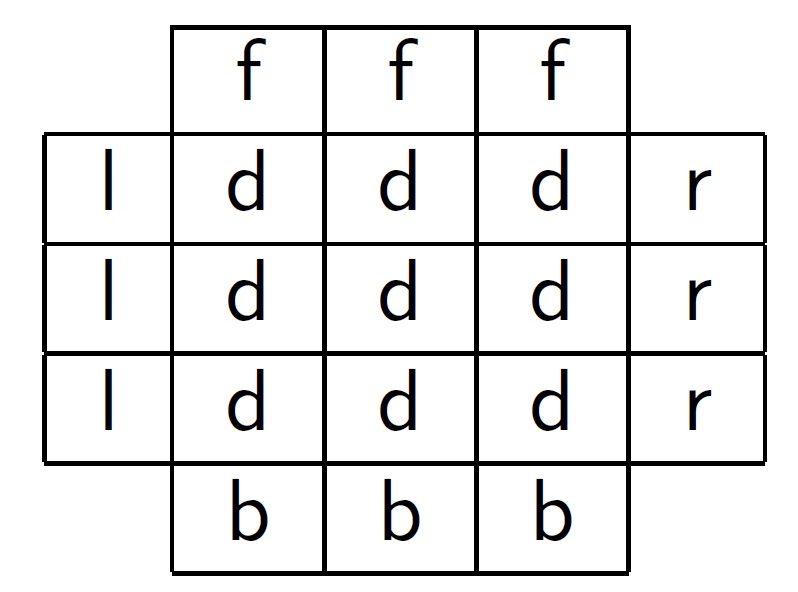
\includegraphics [scale=0.2]{input/pics/rubiks1.jpg}
			\caption{\myCaption{Remember!!}}
	\label{fig:rubiks1}
\end{figure}

Rotate this face clockwise by $90\circ$ (this is called the D move), then the down face looks like:

\begin{figure}[h]
	\centering
		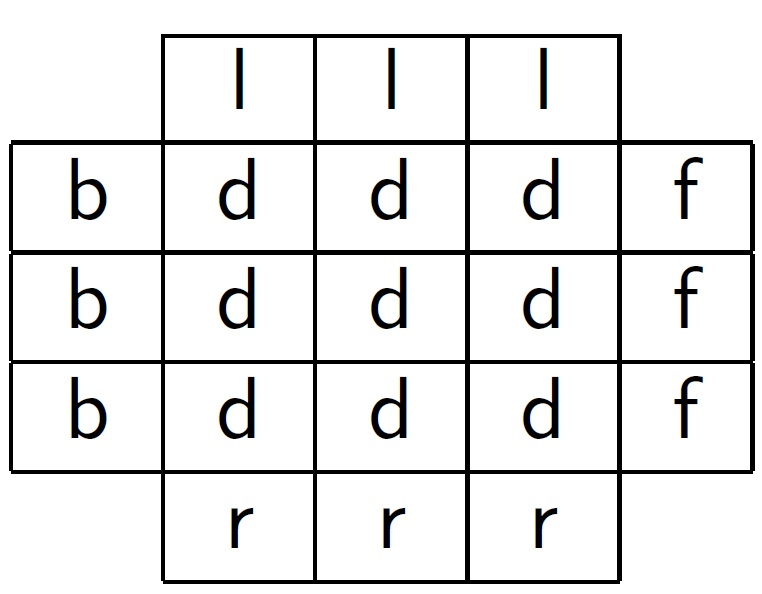
\includegraphics[scale=0.2]{input/pics/rubiks2.jpg}
		\caption{\myCaption{Remember!!}}
	\label{fig:rubiks2}
\end{figure}

So, $D(dlf) = dfr$ because the $dlf$ \cpiece{} now lives in the $dfr$ cubicle (with the down face of the \cpiece{} lying in the down
face of the cubicle, the left face of the \cpiece{} lying in the front face of the cubicle, and the front face of the \cpiece{} lying
in the right face of the cubicle). Similary, $D(dfr) = drb$, $D(drb) = dbl$, and $D(dbl) = dlf$. Do the same thing
for the edge \cpiece{}s, and then $D = (dlf dfr drb dbl)(df dr db dl)$.

\section{Configurations of the Rubik's Cube}

A configuration of the \rubik{} is defined by the position and orientation of its edge and corner \cpiece{}s. The corner \cpiece{} positions can be described as an element of $\sigma$ of $S_8$ . This can also be described as the element of $S_8$ that moves the corner \cpiece{}s from their start position to a new position. The edge \cpiece{}s is described as $\tau$ of $S_12$. 

The orientation of the edge and corner \cpiece{}s are described by a given start orientation and a systematic way of describing how a given orientation is different from the start orientation.

\myTail{
}
%\end{document}